\section{Locally Optimized Partial Solution}

Once we have a partial solution, we convert $K$ partitions into $K$ tours using standard TSP algorithm for each partition. In this stage, we define a new type of operation for our local search. \textbf{Transfer2} is the operation of transferring a node from the longest tour to another edge of a shorter tour. We perform the custom local search algorithm below to optimize both objectives maximum of tour cost and sum of tour cost.

\begin{figure}[h!]
\centering
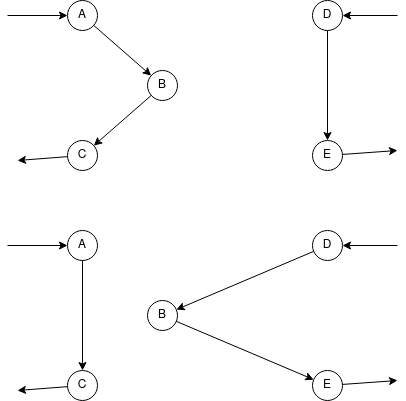
\includegraphics[width=0.8\textwidth]{assets/transfer2.png}
\caption{Transfer of $B$ to $D \to E$}
\label{fig:transfer2}
\end{figure}


\begin{algorithm}[H]
\caption{Local Search 2}
\label{algo:localsearch2}
\textbf{Input:}:

    Initial $K$ cycles
    
    \textbf{Strategy} $\in$ \{ \textbf{first}, \textbf{best} \} 

\textbf{Output:}:

    Final $K$ cycles
    
\textbf{Procedure:}:

\textbf{While} \textbf{true}:

    \hspace{1cm} \textbf{var} \textbf{candidate\_set} = []

    \hspace{1cm} \textbf{For} operation \textbf{in} all possible operations:
    
        \hspace{2cm} Calculate the gain of the operation
            
        \hspace{2cm} \textbf{If} operation reduced maximum of tour cost:
            
            \hspace{3cm} \textbf{Push} the operation and gain to candidate set
                
            \hspace{3cm} \textbf{If} \textbf{Strategy} is \textbf{first}:
                
                \hspace{4cm} \textbf{break}
                
    \hspace{1cm} \textbf{If} \textbf{candidate\_set} is empty:
    
        \hspace{2cm} \textbf{break}
    
    \hspace{1cm} Pick the candidate with smallest sum of tour cost, update the current $K$ partitions
    
\textbf{return} current $K$ partitions

\end{algorithm}

Performing this algorithm with strategy \textbf{best} guarantees to find a locally best partition. Equivalently, if a partial solution is returned by this algorithm, among its neighbourhood defined by the operation \textbf{Transfer2}, there is no other partial solution has a better maximum of tour cost and there is no other partial solution has a better sum of tour cost without scarifying the maximum of tour cost.


\begin{figure}[h!]
\centering
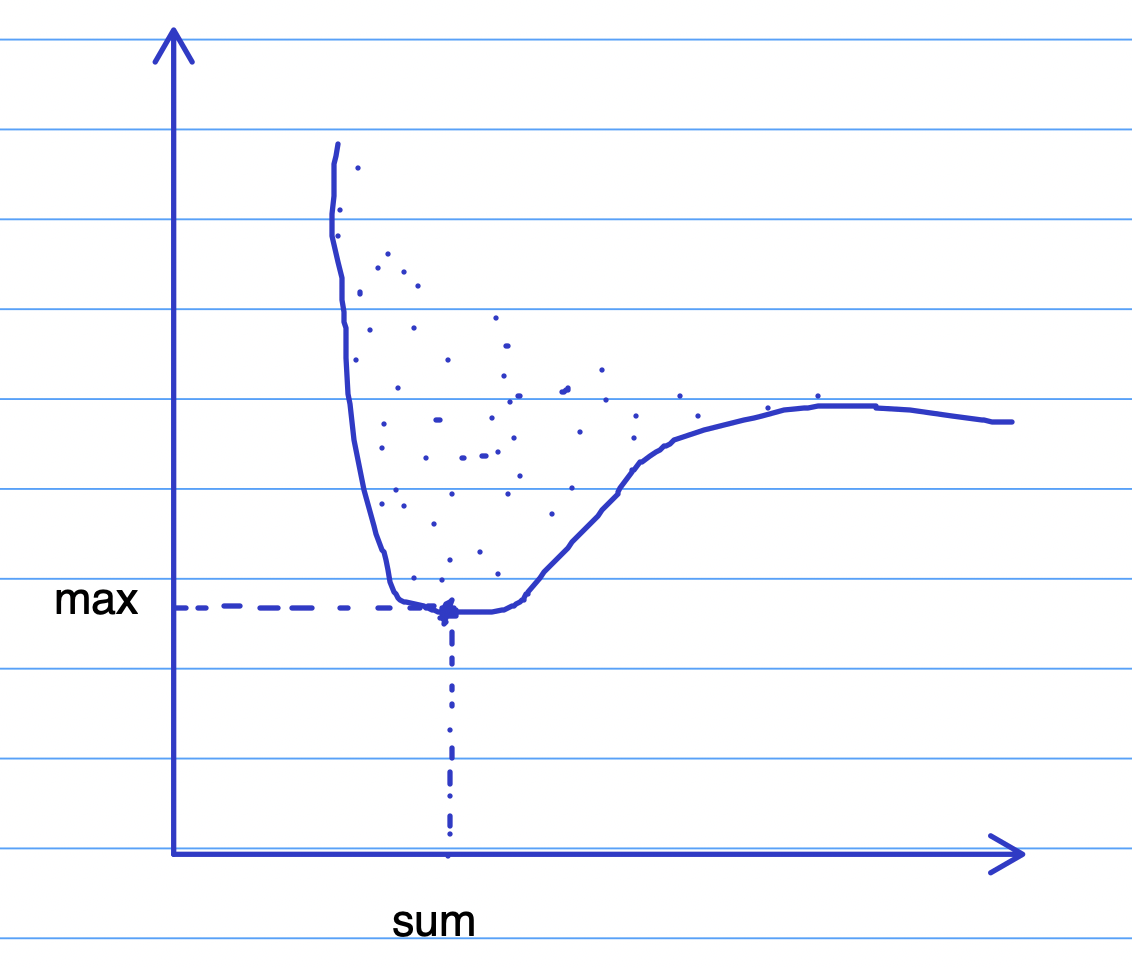
\includegraphics[width=0.8\textwidth]{assets/multiobjective.png}
\caption{Multi-objective analogy}
\label{fig:multiobjective}
\end{figure}
